\chapter{Anwendungsbeispiele}   
Dieses Kapitel gliedert sich in verschiedene Unterkapitel, in denen jeweils einzelne Anwendungsbeispiele der Singulärwertzerlegung näher beschrieben werden.
In ausgewählten Beispielen wird zusätzlich mithilfe der Programmiersprache \texttt{Python} eine eigene, simplifizierte Art der Anwendung konstruiert.
Grundkenntnisse in \texttt{Python} werden bei den Erklärungen des Programmcodes vorausgesetzt, es wird folglich nicht auf jede Zeile im Code genau eingegangen.

\section{Hauptkomponentenanalyse}

Die Hauptkomponentenanalyse (engl.\ \textit{Principal Component Analysis}, PCA) ist ein Verfahren zur Dimensionsreduktion von Daten.
Genauer: Es handelt sich um eine Methode, um komplexe Daten auf ihr Wesentliches zu reduzieren, was eine Weiterverarbeitung und Visualisierung erleichtert.

In diesem Unterkapitel wird zunächst die Intuition hinter der PCA erläutert, bevor der mathematische Hintergrund und insbesondere die Verbindung zur Singulärwertzerlegung beschrieben wird.
Abschließend betrachten wir ein konkretes Anwendungsbeispiel und berechnen dies mithilfe von \texttt{Python}.

\subsection{Intuition der PCA}
Angenommen, es sei eine Datenmatrix
\begin{equation*}
    \big[
        \begin{matrix}
            x_1 \dots x_n
        \end{matrix}    
    \big] \in \R^{m \times n},
\end{equation*}
gegeben, wobei die Spaltenvektoren \(x_i \in \R^{m}\) für \(i \in \{1,\ldots,n\}\) die Ausprägung von \(n\) Merkmalen über \(m\) Objekte hinweg repräsentieren.
In \zcref{fig:pcadim}, zu finden in \zcref{appen}, wird dies für verschiedene Werte von \(n\) veranschaulicht.
Soll die Ähnlichkeit der Objekte hinsichtlich der unterschiedlichen Merkmale betrachtet werden, kann dies im zwei- und dreidimensionalen Raum durch die grafischen Darstellungen erfolgen, indem die Entfernung der verschiedenen Punkte analysiert wird.
In höheren Dimensionen ist diese visuelle Interpretation jedoch nicht mehr möglich, es besteht also die Notwendigkeit, die Anzahl der Merkmale zu verringern.

Die Hauptkomponentenanalyse bietet dafür die Möglichkeit, indem neue, unkorrelierte Komponenten konstruiert werden, die sich als Linearkombination aus den bestehenden Merkmalen zusammensetzen.
Das Ziel der Analyse ist, die Daten auf eine niedrigere Dimension zu projizieren und gleichzeitig ein Minimum an Informationen zu verlieren, also eine maximale Streuung oder auch Varianz der Daten zu erhalten.
Um dieses Konzept näher zu verdeutlichen, betrachte Abbildung.
\begin{figure}[hbt]
    \centering
    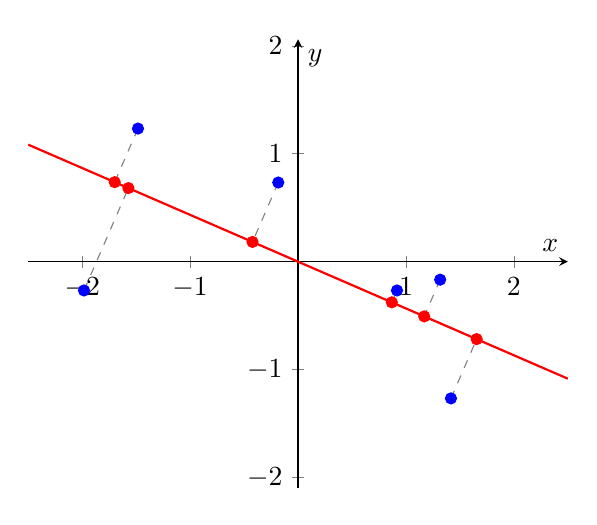
\begin{tikzpicture}[baseline]
        \begin{axis}[
            xlabel={\(x\)},
            ylabel={\(y\)},
            axis y line=center,
            axis x line=middle,
            axis equal,
        ]
        \addplot[only marks,mark options={fill=blue, color=blue},domain=-2:2] coordinates {
            (1.4167,-1.2667)
            (-1.4833,1.2333)
            (1.3167,-0.1667)
            (-1.9833,-0.2667)
            (0.9167,-0.2667)
            (-0.1833,0.7333)                
        };
        \addplot[red, thick, domain=-2.5:2.5] {-0.4337*x};

        \addplot[only marks, mark options={fill=red, color=red}] coordinates {
            ( 1.65481157, -0.71762599)
            (-1.69867778,  0.73664903)
            ( 1.16912424, -0.50700271)
            (-1.57200891,  0.68171777)
            ( 0.86894276, -0.37682593)
            (-0.42195053,  0.18298317)
        };
        \addplot[dashed, gray] coordinates {
            (1.4167, -1.2667) ( 1.65481157, -0.71762599)
        };
        \addplot[dashed, gray] coordinates {
            (-1.4833, 1.2333) (-1.69867778,  0.73664903)
        };
        \addplot[dashed, gray] coordinates {
            (1.3167, -0.1667) ( 1.16912424, -0.50700271)
        };
        \addplot[dashed, gray] coordinates {
            (-1.9833, -0.2667) (-1.57200891,  0.68171777)
        };
        \addplot[dashed, gray] coordinates {
            (0.9167, -0.2667) (0.86894276, -0.37682593)
        };
        \addplot[dashed, gray] coordinates {
            (-0.1833, 0.7333) (-0.42195053,  0.18298317)  
        };
        \end{axis}
    \end{tikzpicture}
\end{figure}
